\documentclass[12pt,twoside]{book}

\usepackage[a4paper,width=150mm,top=25mm,bottom=25mm]{geometry}
\usepackage[utf8]{inputenc}
\usepackage{xcolor}
\usepackage{acronym}
\usepackage{graphicx}
\usepackage{amsmath}
\usepackage{url}

\usepackage{hyperref}
\hypersetup{
    colorlinks,
    linkcolor= [RGB]{8 0 125},
    citecolor= [RGB]{8 0 125},
    urlcolor= [RGB]{8 0 125}
}

\usepackage{fancyhdr}
\pagestyle{fancy}
\renewcommand{\chaptermark}[1]{ \markboth{#1}{} }
\renewcommand{\sectionmark}[1]{ \markright{#1}{} }
\fancyhead[LO, RE]{\thesection~ \rightmark}
\fancyhead[RO,LE]{Chapter \thechapter}
\fancyfoot[C]{\thepage}


\begin{document}


\newgeometry{centering}  
\begin{titlepage}
    \begin{center}
        \vspace*{1cm}
        
        \Huge
        \textbf{Lepton flavour violation in Z boson decays}
        
        \vspace{0.5cm}
        
        \large
        
        von
        
        \vspace{0.5cm}
	
	\textbf{B. Sc.}	
	
	\vspace{0.3cm}
        
        \textbf{David Brunner}
        
        \vspace{4.0cm}
        
        Masterarbeit in Physik
        
        \vspace{0.5cm}
        
        vorgelegt der 
        
        \vspace{0.5cm}
        
        Fakultät für Mathematik, Informatik und Naturwissenschaften der RWTH Aachen
        
        \vspace{0.5cm}
        
        im \today{}
        
        \vspace{0.5cm}
        
        angefertigt am
        
        \vspace{0.5cm}
        
        III. Physikalisches Institut B
        
        \vspace{0.5cm}
        
        bei 
        
        \vspace{0.5cm}
        
        Prof. Dr. Achim Stahl
    
    \end{center}
\end{titlepage}
\restoregeometry

\clearpage{\pagestyle{empty}\cleardoublepage}

%\chapter*{Abstract}
%\thispagestyle{empty}

In the Standard Model of particle physics the $Z$ boson can decay into a pair of leptons with the same flavour. The observation of the Z boson decaying into a pair of leptons with different flavour, namely the decay into a pair of electron/muon, electron/$\tau$ lepton or muon/$\tau$ lepton would violate lepton flavour conservation and would indicate physical processes beyond the Standard Model. \\

Previous searches for lepton flavour violation in Z boson decays set a constraint on the branching ratio on these decays. For the decay into an electron/muon pair the CMS collaboration set the limit to $\text{BR}(Z\to e\mu) < 7.3\cdot 10^{-7}$, for the decay into a pair of electron/$\tau$ lepton and muon/$\tau$ lepton the LEP collaboration set to limit to $\text{BR}(Z\to e\tau) < 9.8\cdot 10^{-6}$ and $\text{BR}(Z\to \mu\tau) < 1.2\cdot 10^{-5}$. \\

In this analysis the data recorded by the CMS detector in 2016 with a center-of-mass energy of $\sqrt{s} = 13$ TeV and a integrated luminosity of $\mathcal{L} = 35.9$ fb$^{-1}$ is analyzed. All three decays channel are analyzed independently in a model independent approach. In the analysis hadronic decaying $\tau$ leptons are considered. For each final state a boosted decision classifier is trained as discriminating variable. With the CL$_s$ method this classifier is analyzed in bins of jet multiplicity to set expected limits on the branching ratios of the lepton flavour violating Z boson decays. The expected limits are set to $\text{BR}(Z\to e\mu) < 2.8\cdot 10^{-7}$,  $\text{BR}(Z\to e\tau) < 2.25\cdot 10^{-5}$ and  $\text{BR}(Z\to \mu\tau) < 8.6\cdot 10^{-6}$. In comparison to the previous analysis, in the $e\mu$ final state this analysis gained a factor three in terms of sensitivity, in the $e\tau$/$\mu\tau$ final state this analysis is as sensitive as the previous analysis from LEP.


\tableofcontents
\thispagestyle{empty}
\clearpage{\pagestyle{empty}\cleardoublepage}

\listoffigures
\thispagestyle{empty}
\addcontentsline{toc}{chapter}{List of figures}
\clearpage{\pagestyle{empty}\cleardoublepage}

\listoftables
\thispagestyle{empty}
\addcontentsline{toc}{chapter}{List of tables}
\clearpage{\pagestyle{empty}\cleardoublepage}

\chapter{Theoretical basics about the Standard Model and lepton flavour violation}
The Standard Model of Particle Physics (SM) is the description of the physics of elementary particles and their interaction, which is known up now. The theoretical foundation is the perturbative quantum field theory (QFT) which is harmonised with Special Relativity. In the formaslim of QFT classical fields are quantized and the information of the interaction of the particles is encoded in the lorentz-invariant lagrangian density $\mathcal{L}$. 

\section{Particles and interactions}
\label{section_1_1}

In the SM elemental particles can be characzerized by their spin, which is a quantum number describing a analogon to the intrinsic angular momentum. Fermions carry spin $\frac{1}{2}$ and are represented by Dirac spinors $\psi$, which are complex 4-component objects defined through their behaviour under Lorentz transformation: $\psi^{\alpha}(x) \rightarrow S[\Lambda]^{\alpha}_{\beta} \psi^{\beta}(\Lambda^{-1}x)$. The interaction between the fermions are described by gauge symmetries, which are local symmetry transformations, leaving the langrangian invariant with the introduction of a gauge boson. Gauge boson are elemental particles with spin 1. All relevant symmetries and the corresponding interaction are described in the following, the list of all elemental particle and their properties are listed in table \ref{tab:1.1}.

\subsection*{\small U(1)${_e}$ symmetry and quantum electrodynamics (QED)}

The free langrangian of a fermion using the Dirac spinors, using $\gamma^{\mu}$ as the gamma matrizes and $\bar{\psi} = \psi^{\dagger}\gamma^{0}$, can be written as:

\begin{equation}
	\mathcal{L}_{0} =  i\bar{\psi}(x)\gamma^{\mu}\partial_{\mu}\psi(x) - m\bar{\psi}(x)\psi(x)
\end{equation}

Performing a global transformation of the the kind $\psi(x) \rightarrow \psi'(x) = e^{iQ\alpha}\psi(x)$, with Q and $\alpha$ as real constants, the langrangian stays invariant under this so called U(1) transformation. The invariance is not fullfilled if $\alpha$ depends explictly on the spacetime $x$ and is called a local gauge transformation. To insure invariance under a gauge transformation, a new 4-component lorentz vector field $A_{\mu}(x)$ is introduced with following property under U(1) transformation: $A_{\mu} \rightarrow A'_{\mu}(x) = A_{\mu}(x) + \frac{1}{e}\partial_{\mu}\alpha(x)$. Using the definition of the covariant derivate $D_{\mu} = \partial_{\mu} - ieQA_{\mu}(x)$, the following langrangian stays invariant under local U(1) transformation:

\begin{equation}
	\mathcal{L} = i\bar{\psi}(x)\gamma^{\mu}D_{\mu}\psi(x) - m\bar{\psi}(x)\psi(x) = \mathcal{L}_{0} + eQA_{\mu}(x)\bar{\psi}(x)\gamma^{\mu}\psi(x)
\end{equation}

With the gauge transformation the gauge boson of the electromagnetic interaction is introduced, which couples to the fermions with electric charge e: the photon $\gamma$.


\subsection*{\small SU(3)${_C}$ symmetry and quantum chromodynamics (QCD)}

Beside the electric charge, the so-called quarks are fermions carrying the one of three possible color charges (denoted with r,b,g). Labeling the quark spinor with color $c$ as $q^{c} = \psi_{q}(c)$ and putting them all into a three vector with quark $q_{f} = (q^{b}, q^{r}, q^{g})$, the free lagrangian of quarks can be written as

\begin{equation}
	\mathcal{L}_{0} = \sum_{f} \bar{q_{f}}(i\gamma^{\mu}\partial_{\mu} - m_{f})q_{f}
\end{equation}

The index $f$ denotes the flavour of the quark is explained below. Like in the QED example a local gauge theory exists, which introduces gauge bosons. A transformation of the kind $q_{f} \rightarrow q'_{f} = e^{i\frac{\lambda^{a}}{2}\alpha_{a}(x)} q_{f}$, with $\frac{1}{2} \lambda^{a}$ as non communting 3x3 matrixes and $a \in (1, 2, .., 8)$, is a local SU(3)$_{C}$ transformation. To get a lagrangian invariant under this tranformation, 8 new gauge bosons $G^{\mu}_{a}(x)$, so-called gluons have to be introduced, corresponding to the number of generators $\lambda^{a}$ to represent the SU(3)$_{C}$ algebra. Defining the covariant derivative $D_{\mu} = \partial_{\mu}-ig_{s}\frac{\lambda^{a}}{2}G^{\mu}_{a}(x)$ and demand the gluons to transform using $U = e^{i\frac{\lambda^{a}}{2}\alpha_{a}(x)}$ like $G^{\mu}_{a}(x) \rightarrow G^{\mu}(x)' = UG^{\mu}U^{\dagger} - \frac{i}{g_s}(\partial^{\mu}U)U^{\dagger}$ the invariant lagrangian of QCD can be written like 

\begin{equation}
	\mathcal{L} = \sum_{f} \bar{q_{f}}(i\gamma^{\mu}D_{\mu} - m_{f})q_{f}
\end{equation}


\subsection*{\small SU(2)$_{W}$ x U(1)$_{Y}$, the electroweak interaction and Higgs mechanism}

The flavour of fermions is a quantum number describing of the type particle. For the quarks six different flavours (up, down, charm, strange, top, bottom) exist, for the color-less leptons/neutrinos fermions the three lepton flavour (electron, muon, tau) exist. Also a important quantity is the chirality, because in the electroweak theory not all chirality configuration of the fermions couples to the gauge bosons. We define the spinors of fermions with lefthanded(L) or righthanded(R) chirality with $\psi_{L/R} = \frac{1}{2}(1\mp \gamma^{5})\psi$ and for simplizity looking only at the first generation of quarks/leptons, the spinor of quarks/leptons are defined as $u = \psi_{u}, d = \psi_{d}, e = \psi_{e}, \nu = \psi_{\nu_{e}}$. If the fermions are assembled as $q_{L} = (u_{L}, d_{L}), u_{R}, d_{R}, l_{L} = (e_{L}, \nu_{L}), e_{R}$ and consindering them to be massless, the free langrangian of the electroweak theory is


\begin{equation}
	\mathcal{L}_{0} = i\bar{q}_{L}\gamma^{\mu}\partial_{\mu}q_{L} + i\bar{l}_{L}\gamma^{\mu}\partial_{\mu}l_{L} + \sum_{f \in (e, u, d)} i\bar{f}_{R}\gamma^{\mu}\partial_{\mu}f_{R}
\end{equation}

The local SU(2)$_{W}$ x U(1)$_{Y}$ gauge transformation, which is a tranformation of the kind


\begin{equation}
	\begin{split}
		q_{L} \rightarrow q'_{L} = e^{iQ_{q} \alpha_{Y}(x)} e^{i\frac{\sigma_{j}}{2}\alpha^{j}_{W}(x)}q_{L} \\
		l_{L} \rightarrow l'_{L} = e^{iQ_{l} \alpha_{Y}(x)} e^{i\frac{\sigma_{j}}{2}\alpha^{j}_{W}(x)}l_{L} \\
		f_{R} \rightarrow f'_{R} = e^{iQ_{f} \alpha_{Y}(x)}, \quad f \in (e, u, d)
	\end{split}			
\end{equation}


with $\sigma_{j}, j \in (1,2,3)$ as the Pauli matrices, $Q$ as real constant and $a_{Y}, a^{j}_{W}$ as real function of spacetime, introduces 4 gauge bosons, the three $W^{j}_{\mu}(x)$, origating from SU(2)$_{W}$, and the $B_{\mu}$ from U(1)$_{Y}$. Using $U_{L} = e^{i\frac{\sigma_{j}}{2}\alpha^{j}_{W}(x)}$, demanding the transformation properties $B_{\mu} \rightarrow B'_{\mu} = B_{\mu} + \frac{1}{g'}$, $W'_{\mu} \rightarrow U_{L}\frac{\sigma_{j}}{2}W_{\mu}^{j}U_{L}^{\dagger} - \frac{i}{g}(\partial_{\mu}U_{L})U_{L}^{\dagger}$ and defining the covariante derivate 

\begin{equation}
	\begin{split}
		D^{q}_{\mu} = \partial_{\mu}  - ig\frac{\sigma_{j}}{2}W^{j}_{\mu} - ig'Q_{q}B_{\mu} \\
		D^{l}_{\mu} = \partial_{\mu}  - ig\frac{\sigma_{j}}{2}W^{j}_{\mu} - ig'Q_{l}B_{\mu} \\
		D^{f_R}_{\mu} = \partial_{\mu}  - ig'Q_{f}B_{\mu}, \quad f \in (e, u, d)
	\end{split}
\end{equation}

the gauge invariant lagrangian of the electroweak can be written as 

\begin{equation}
	\mathcal{L} = i\bar{q}_{L}\gamma^{\mu}D_{\mu}^{q}q_{L} + i\bar{l}_{L}\gamma^{\mu}D_{\mu}^{l}l_{L} + \sum_{f \in (e, u, d)} i\bar{f}_{R}\gamma^{\mu}D^{f_R}_{\mu}f_{R}
\end{equation}

The problem from this formulation arises from the fact, that the gauge bosons and fermions are measured to have a mass. To explain this discrepancy the Higgs mechanism is introduced. Considering a complex scalar field doublet $\Phi(x) = (\phi^{1}(x), \phi^{2}(x))$, which transform under SU(2)$_{W}$ like $\Phi(x) \rightarrow \Phi'(x) = e^{iQ_{\Phi} \alpha_{Y}(x)} e^{i\frac{\sigma_{j}}{2}\alpha^{j}_{W}(x)}\Phi(x)$ the lagrangian can be written as

\begin{equation}
	\mathcal{L}_{H} = i\bar{q}_{L}\gamma^{\mu}D_{\mu}^{q}q_{L} + i\bar{l}_{L}\gamma^{\mu}D_{\mu}^{l}l_{L} + \sum_{f \in (e, u, d)} i\bar{f}_{R}\gamma^{\mu}D^{f_R}_{\mu}f_{R}
\end{equation}

\clearpage{\pagestyle{empty}\cleardoublepage}

\chapter{Experimental set up}
In this thesis the data, which is analyzed for the search of \gls{LFV} in Z boson decays, is produced by proton-proton-collisions of the Large Hadron Collider (\gls{LHC}) \cite{LHC} and recorded by the Compact Muon Solenoid (\gls{CMS}) \cite{CMS} in the year of 2016. Both apparatus are explained in the sections \ref{sec:section_2_1} and \ref{sec:section_2_2} respectively and proton physics is explained in section \ref{sec:section_2_1_2}.


\section{Large Hadron Collider}
\label{sec:section_2_1}

The \gls{LHC} is a circular proton-proton-collider with a center of mass energy of $\sqrt{s} = 13$ TeV \cite{LHC2}, which is located at the European Organization for Nuclear Research (\gls{CERN}) in Geneva. A schematic overview of the acceleration system is shown figure \ref{fig:fig_2_1}. The acceleration of the protons is done by a system of pre-accelerators, which feeds the protons then in the \gls{LHC}, where they are further accelerated to reach the designed center of mass energy. \\

\begin{figure}[ht]
	\centering
	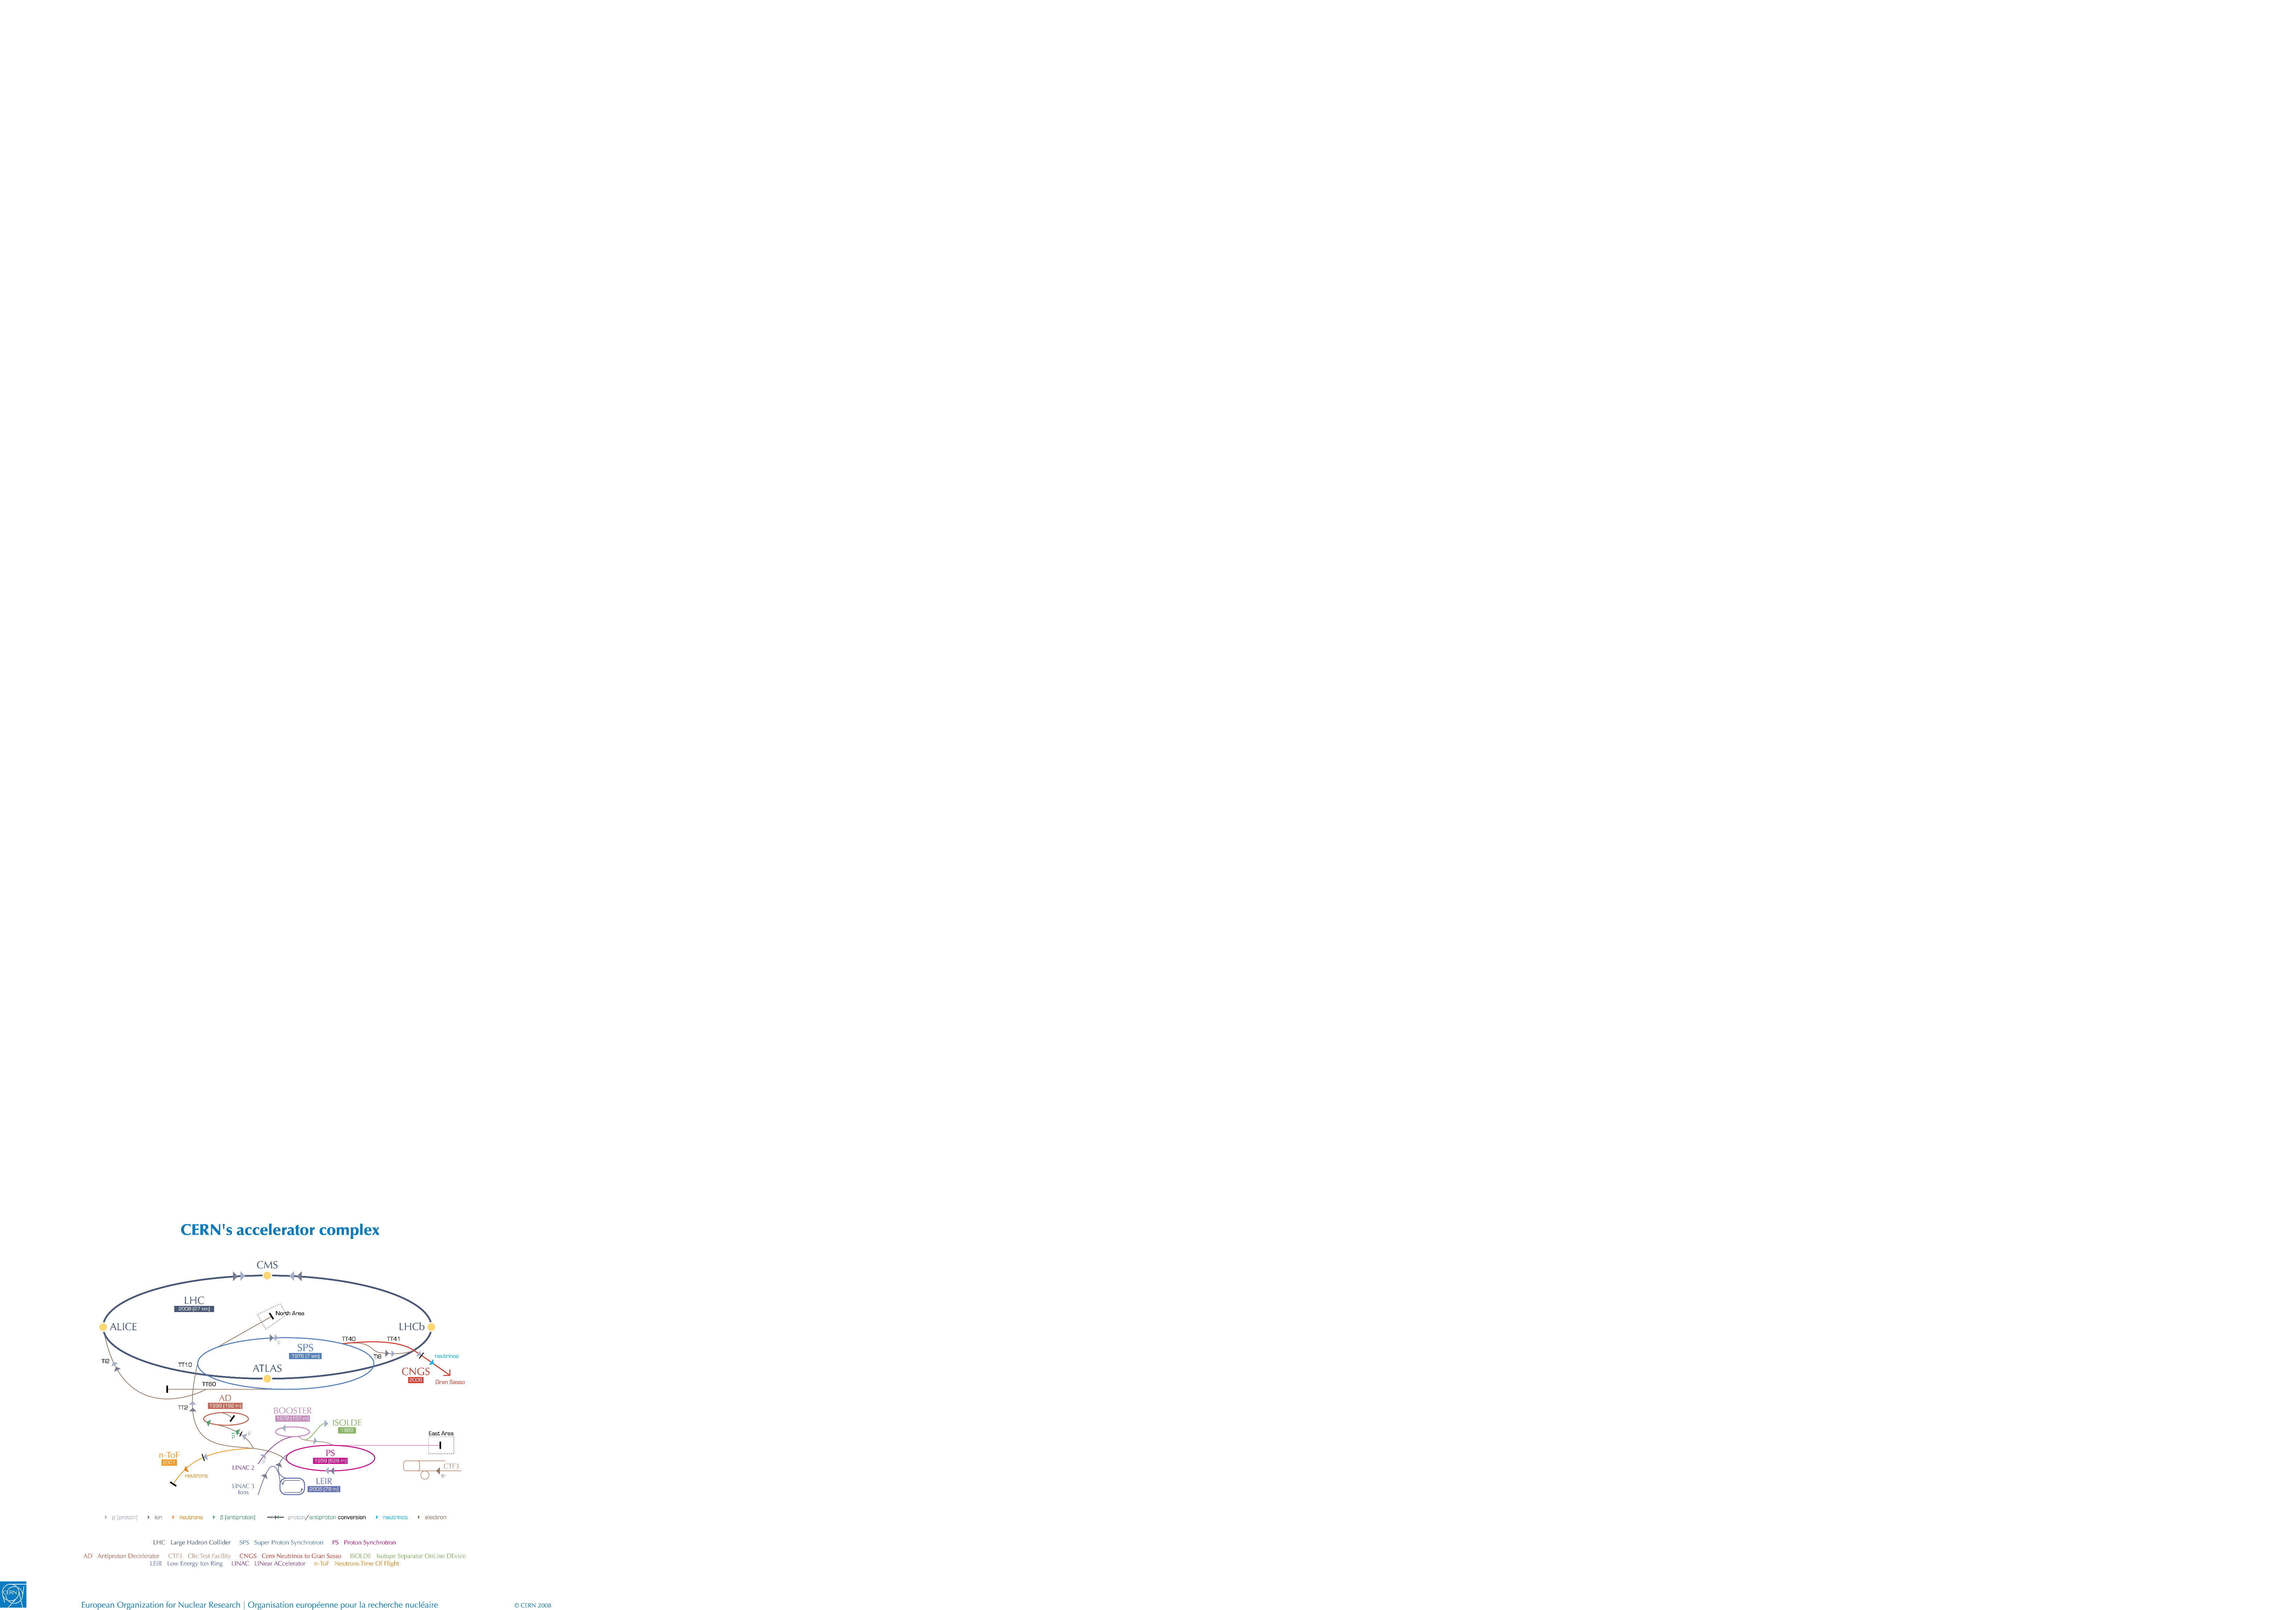
\includegraphics[width=1.0\textwidth]{pictures/LHC.pdf}

	\caption[Schematic overview of CERN accelerator complex]{Schematic overview of \gls{CERN} accelerator complex, including the \gls{LHC} and the previous pre-accelerators. The yellow points mark the position of the particles detectors at the collisions points. Taken from \cite{LHCACCL}.}
	\label{fig:fig_2_1}
\end{figure}

At each collision point of the proton beams a sophisticated detector is installed, indicated by the yellow dots in figure \ref{fig:fig_2_1}. The design of each of these detectors is optimized to a certain physics program. The four big experiments are the \gls{CMS} and A Toroidal LHC Apparatus (\gls{ATLAS}) \cite{ATLAS}, which are designed to probe \gls{SM} and \gls{BSM} physics, the Large Hadron Collider beauty (\gls{LHCb}) \cite{LHCb}, which is designed for decays of hadrons involving bottom quarks, and the A Large Ion Collider Experiment (\gls{ALICE}) \cite{ALICE}, which is designed for heavy ion collisions.


\subsection{Properties of the proton beams}
\label{sec:section_2_1_1}

The protons in the \gls{LHC} are accelerated in bunches, which contain around $10^{11}$ protons, and are separated in space by a time interval of 25 ns \cite{LHCSTATS}. The size of the bunches is oscillating due to dynamics of the charged protons in the magnetic system of the \gls{LHC} \cite{LHC}. The beam size can be parametrized by the emittance $\epsilon$, which describes the spread of the beam particles in the spatial and momentum phase space, and the $\beta$ function, which describes the oscillation amplitude \cite{BEAMPHY}. The properties of the beam have a high impact on the quality of the collider, which is parametrized by instantaneous luminosity $\mathcal{L}$ \cite{Luminosity}

\begin{equation}
	\label{eq:eq_2_1}
	\mathcal{L} = \frac{\gamma \cdot f \cdot k_{b} \cdot n_{1} \cdot n_{2}}{4 \cdot \pi \cdot \epsilon \cdot \beta}
\end{equation} 

with Lorentz gamma factor $\gamma$, the revolution frequency $f$ of the bunches, the number of colliding bunches $k_{b}$ and the number of protons $n_{i}$ in each bunch. There is a direct dependence of rate of collision events $\frac{dN}{dt}$ to the luminosity, and the total number of collision events $N$ to the integrated luminosity $\mathcal{L}_{int}$

\begin{equation}
	\label{eq:eq_2_2}
	\begin{split}
		\frac{dN}{dt} = \sigma \cdot \mathcal{L} \\
		N = \sigma \cdot \mathcal{L}_{int}
	\end{split}
\end{equation}	

with $\sigma$ as the cross section of of a certain process in proton-proton collisions. So the beam parameter have a direct influence on the total number of possible recorded events and the amount statistics which is provided for the analysis. Figure \ref{fig:fig_2_2} shows of the collected integrated luminosity as a function of time during  data-taking run in 2016. 

\begin{figure}[ht]
	\centering
	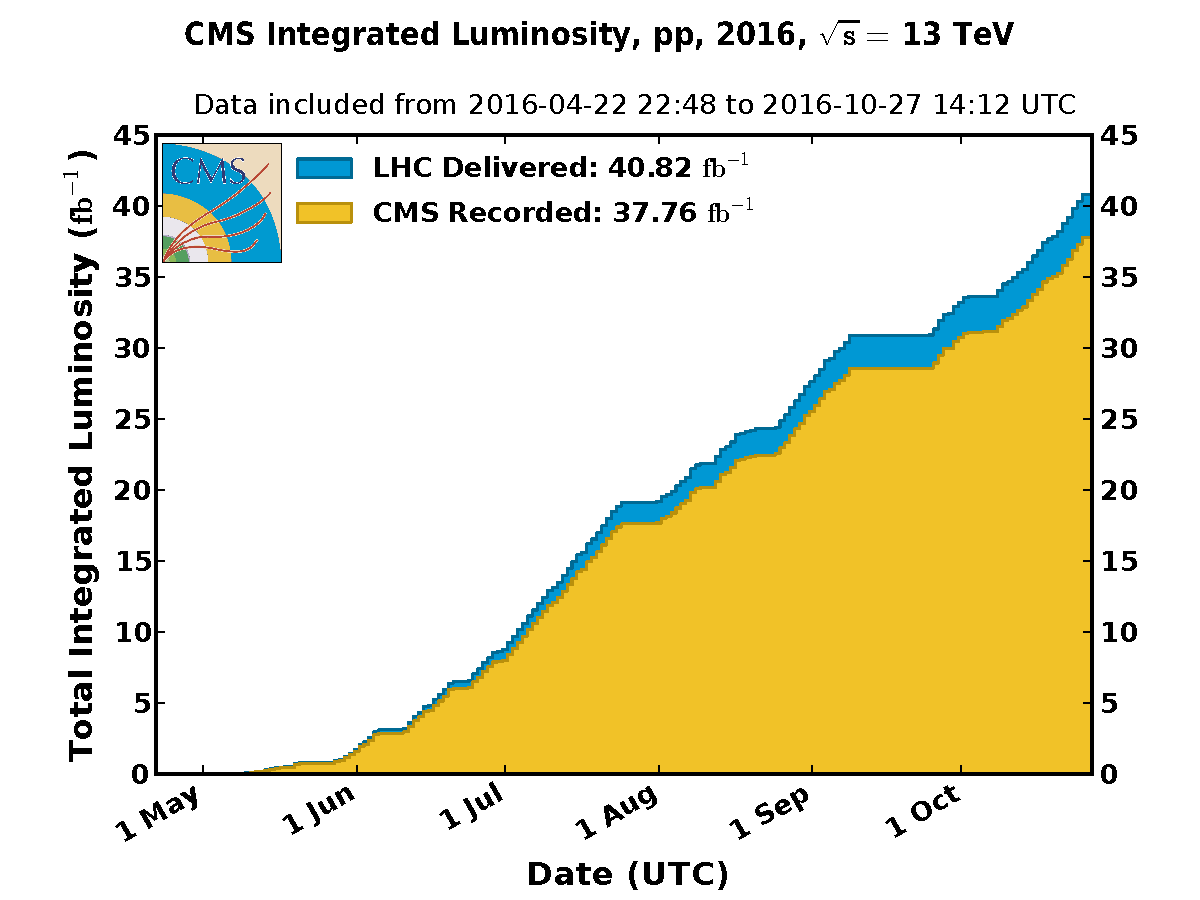
\includegraphics[width=0.7\textwidth]{pictures/int_lumi_per_day_cumulative_pp_2016.pdf}

	\caption[Total integrated luminosity of the year 2016]{Total integrated luminosity collected by \gls{CMS} as a function of time in the run in the year 2016, taken from \cite{CMSLUMI}}
	\label{fig:fig_2_2}
\end{figure}


\subsection{Proton-proton collisions}
\label{sec:section_2_1_2}

Protons are non-elementary hadrons, which are a bound state of three quarks, in this case of two up-quarks and one down-quark. This bound state can be described by \gls{QCD}, see section \ref{sec:section_1_1_2}, and give rise to the quark-parton model \cite{Peskin}. In this description protons are composite of the partons, which are beside the three quarks of the bound state, other quarks and gluons which are produced/annihilated during the interaction in the bound state. Each of the quarks and gluons carry a fraction $x_{i}$ of the total momentum $P$ of the proton, and the probability of an existing parton with flavour f, with $f \in (u, d, \bar{u}, \bar{d}, ... g)$ and with $x_{i}$ is described by the parton density function (\gls{PDF}) $f_{f}(x)$ \cite{Peskin, PDF1}. \gls{PDF} are not predictable by \gls{QCD} and have to be measured in deep inelastic scattering processes. As an example, figure \ref{fig:fig_2_3} shows the measurement of the \gls{PDF} in the ZEUS experiment \cite{ZEUS}. \\

\begin{figure}[ht]
	\centering
	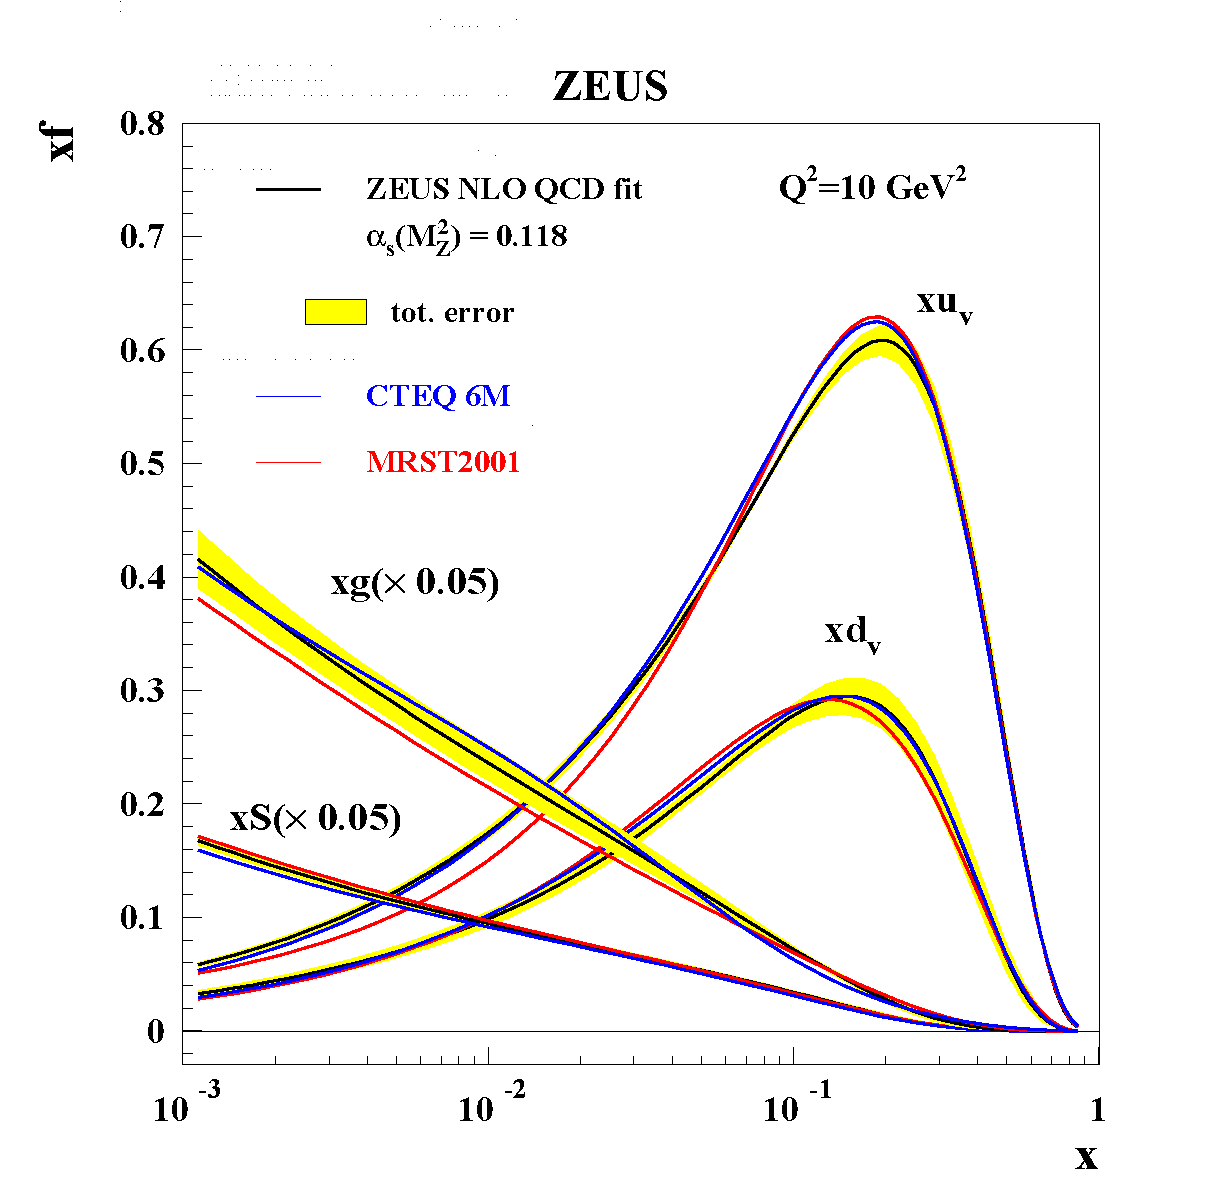
\includegraphics[width=0.7\textwidth]{pictures/ZEUS_PDF.pdf}

	\caption[Proton \gls{PDF} from ZEUS]{\gls{PDF} of up-quarks, down-quarks and gluons in a proton measured by the ZEUS experiment, taken from \cite{PDFMEAS}. The measurement shows that $u$ and $d$ quarks, which are in the bound state of the proton, have a high probability to carry a large fraction of the proton momentum. Other quarks and gluons have a high probability to carry a low momentum fraction of the proton.}
	\label{fig:fig_2_3}
\end{figure}

In collisions of the protons at the \gls{LHC} the cross sections of the different processes depend on the \gls{PDF} and the $x_{i}$ of the partons. Taking as example proton-proton collisions into fermion pair production, two quarks with momentum $x_{1}P$ and $x_{2}P$ will produce the fermion pair, all the other constituent $X$ are not participating in the interaction and carry away the remaining proton momenta, see figure \ref{fig:fig_2_4} for a schematic example. The cross section $\sigma(pp\to f\bar{f} + X)$ \cite{Peskin} for such a process can be calculated with 

\begin{equation}
	\label{eq:eq_2_3}
	\sigma(pp\to f\bar{f} + X) = \int_{0}^{1}dx_{1}\int_{0}^{1}dx_{2}\sum_{f \in (u, d, \bar{u}, \bar{d}, ... g)} f_{f}(x_{1})f_{\bar{f}}(x_{2}) \cdot \sigma(q_{f}(x_{1})q_{\bar{f}}(x_{2}) \to f\bar{f}). 
\end{equation}


\begin{figure}[ht]
	\centering
	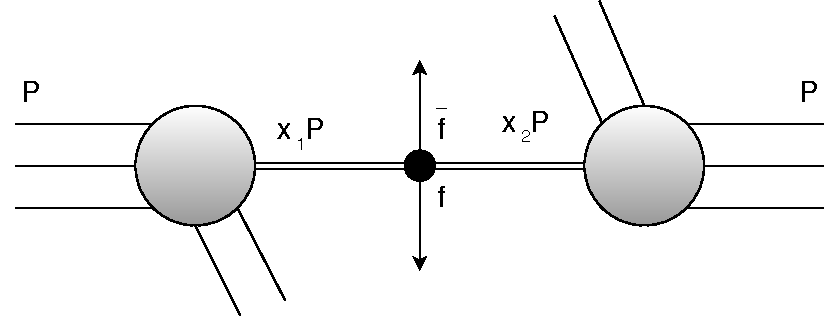
\includegraphics[width=0.7\textwidth]{pictures/ppcollision.pdf}

	\caption[Sketch of proton-proton collision]{Sketch of a proton-proton collision at the \gls{LHC}. The protons have momentum $P$, the quarks involved in the interaction have the fraction $x_{i}$ of it, all other rest carries away the remaining momenta}
	\label{fig:fig_2_4}
\end{figure}


\section{Compact Muon Solenoid}
\label{sec:section_2_2}

The \gls{CMS} is a multi-purpose, multi-functional particle detector. The detector consists of several layers, which have each its functionality and purpose for the detection of particles. This design enables the measurement of kinematic properties of the particles produced in each scattering event, like momenta/energy/angular distributions, and the identification of the particles. Figure \ref{fig:fig_2_5} shows the \gls{CMS} profile with all detector layers, which are explained in section \ref{sec:section_2_2_2}, and the interactions of different particle species in the detector, which are explained in section \ref{sec:section_2_2_4}.

\begin{figure}[ht]
	\centering
	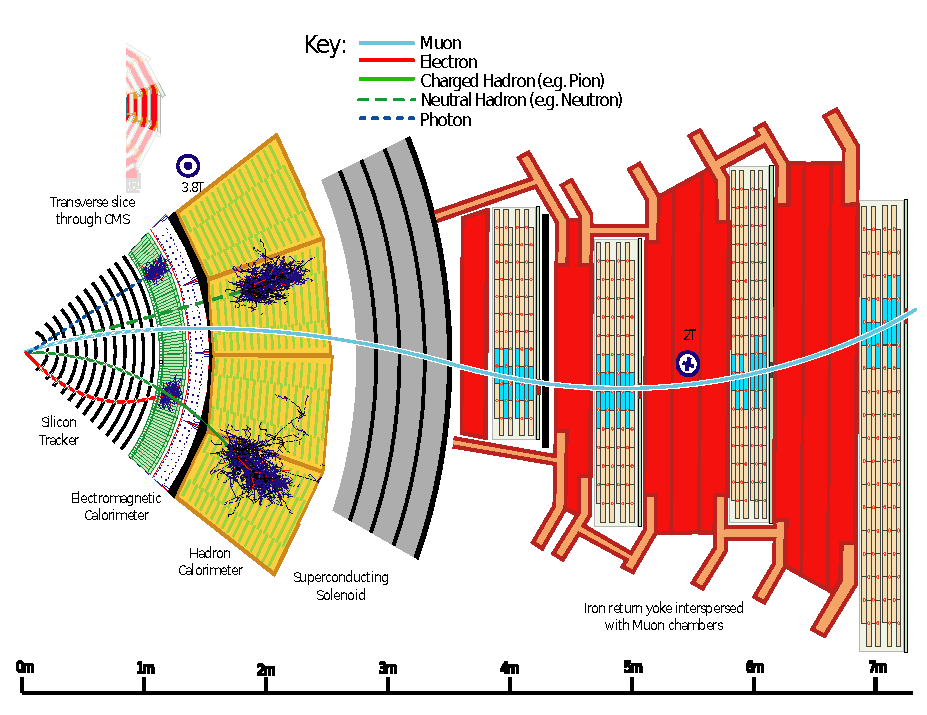
\includegraphics[width=0.7\textwidth]{pictures/CMS.pdf}

	\caption[Profile of CMS detector]{Sketch of the profile of \gls{CMS} with detectors and several particle species and their interactions in the detectors, taken from \cite{PARTICLEFLOW}}
	\label{fig:fig_2_5}
\end{figure}


\subsection{Coordinate convention}

The coordinate system is set to have the origin centered at the nominal collision point of the detector, with the x-axis pointing into the direction of the center of \gls{LHC}, the y-axis is pointing upwards into direction of the sky and z-axis points into the direction of the beam pipe. The coordinate system is choosen in a way, that the azimuthal angle $\phi$ is measured in the x-y plane, and the polar angle $\theta$ is measured from the z-axis. Instead of the polar angle $\theta$, in general the pseudo rapidity \gls{eta} $= -\ln{\tan{\frac{\theta}{2}}}$ is used due to the invariance under lorentz boost of $\Delta$\gls{eta} of two objects in the high energy limit.


\subsection{Sub-detectors of \gls{CMS}}
\label{sec:section_2_2_2}

\subsection*{Tracker system}

The most inner part of \gls{CMS} is the silicon tracker \cite{CMS2, CMSTRACKER}. Its inner part is the pixel detector, which is cylindrical around the beam. Figure \ref{fig:fig_2_6} shows the layout of the pixel detector. It consists of three layers in the barrel, which are located at the radial distance of 4.4 cm, 7.3 cm, 10.2 cm and have a length of 53 cm, and two turbine shaped layers on each side of the barrel, which are located $|z| = 34.5/46.5$ cm and have a radial expansion of 6 to 15 cm. All in all $66\cdot 10^{6}$ pixels with a size of 100 x 150 $\mu$m$^{2}$ are implemented in the pixel detector. The precision of the space point measurement of a crossing charged particle is about 10 $\mu$m in the $r-\phi$ direction and 20 $\mu$m in the z direction. \\

\begin{figure}[ht]
	\centering
	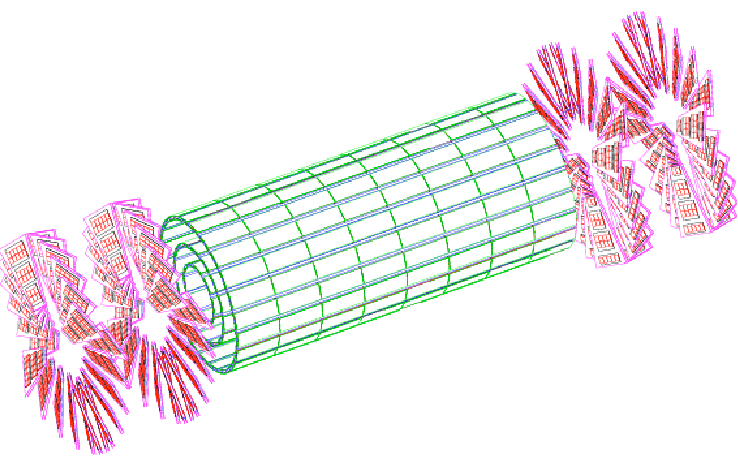
\includegraphics[width=0.7\textwidth]{pictures/CMS_tracker.pdf}

	\caption[Pixel detector layout of CMS]{Pixel detector layout of CMS, taken from \cite{CMS2}}
	\label{fig:fig_2_6}
\end{figure}


The outer part of the tracker is the silicon strip detector as shown in figure \ref{fig:fig_2_7}. The strip detector is spaced in cylindric layers around the beam pipe and is divided into an inner/outer barrel and the inner disc and endcap. The inner barrel is made of 4 layers with a coverage in z direction up to 65 cm in each direction, with a strip thickness of 320 $\mu$m and a $r-\phi$ resolution of 23-34 $\mu$m and z resolution of 23 $\mu$m. The outer barrel includes six layers with a strip thickness of 500 $\mu$m, a coverage in z direction up to 110 cm and a $r-\phi$ coordinate resolution of 35-52 $\mu$m and z coordinate resolution of 52 $\mu$m. The endcap are nine disc-like layers on each side in z direction, occupying the space in the range 120 cm $< |z| < $ 280 cm, the inner discs are arranged in 3 layers and fill the gap between barrel and endcap. In total a region up to $|$\gls{eta}$|$ $< 2.5$ is covered by the complete strip detector. \\

\begin{figure}[ht]
	\centering
	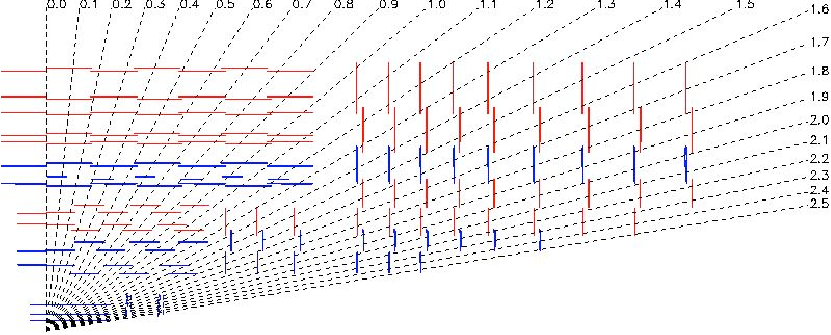
\includegraphics[width=1\textwidth]{pictures/CMS_strip.pdf}
	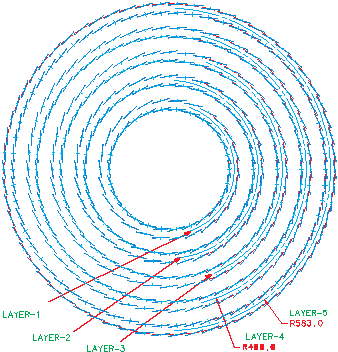
\includegraphics[width=0.5\textwidth]{pictures/CMS_strip2.pdf}

	\caption[Strip detector of CMS]{The first subfigure shows the layout in a z-view, where the numbers give the $\eta$ region. The second subfigure shows a transverse view of the barrel strip detector, taken from \cite{CMS2, ECAL}}
	\label{fig:fig_2_7}
\end{figure}

\subsection*{Calorimeter}

Outside the tracker two calorimeters are installed. The electromagnetic calorimeter (\gls{ECAL}) \cite{CMS2, ECAL} is built up by 61200 lead tungstate (\gls{PbWO4}) crystals in the barrel part and 7324 crystals in the endcap. Figure \ref{fig:fig_2_8} shows the schematic view of the \gls{ECAL}. The barrel region covers a region from 0 $<$ $|$\gls{eta}$|$ $<$ 1.479, in which each crystal have the dimensions of 22 mm x 22 mm x 230 mm. The endcap region covers to remaining part of 1.479 $<$ $|$\gls{eta}$|$ $<$ 3.0, in which the crystals have a dimension of 28.6 mm x 28.6 mm x 220 mm. In $r$ direction the barrel region is located at a distance to the beam pipe of 129 cm, the endcap region is located at a distance of 314cm. For the readout the scintillation light, due to of energy deposition of the particles in the barrel region silicon avalanche photo-diodes are used, in the endcap vacuum phototrides are used. The energy resolution of the \gls{ECAL} is given by

\begin{equation}
	\label{eq:eq_2_4}
	\frac{\sigma}{E} = (\frac{3.63 \sqrt{\text{MeV}}}{\sqrt{E}})^2 + (\frac{124 \text{MeV}}{\sqrt{E}})^2 + 0.26^{2}
\end{equation}

and measured for supermodules, which group 4 modules, which contains 500 crystals each. \\

\begin{figure}[ht]
	\centering
	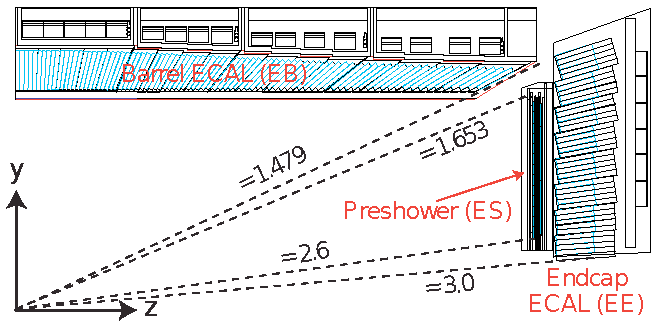
\includegraphics[width=1\textwidth]{pictures/CMS_ElectromagneticCalorimeter.pdf}

	\caption[Electromagnetic calorimeter of CMS]{Schematic view of the \gls{ECAL}, taken from \cite{CMS2}}
	\label{fig:fig_2_8}
\end{figure}

The second calorimeter is the hadronic calorimeter (\gls{HCAL}) \cite{CMS2, HCAL}. It is build up by wedges made of brass absorber plates, orientated parallel to the beam axis, with plastic scintillators between each absorber plate. The placement of absorber/scintillator is alternating, in total 17 layers of active scintillator material are placed, which are connected with a wavelength shifting fiber, forming so-called towers. The readout of the optical signal from the HCAL towers is done by pixelated hybrid photodiodes. The \gls{HCAL} is divided into a barrel region with $|$\gls{eta}$|$ $< 1.3$, with 32 towers, and the endcap region covering the region of 1.3 $<$ $|$\gls{eta}$|$ $<$ 3.0 with 14 towers. In addition, an outer hadron calorimeter located outside the magnet coil in front of the muon chambers is installed. It is assembled in 5 rings placed by a distance of 2.54 m in z-direction, covering a region of $|$\gls{eta}$|$ $< 1.24$, where the ring are made of a layer of iron and scintillator material. Figure \ref{fig:fig_2_8} shows a schematic overview of the tower assembly. \\

\begin{figure}[ht]
	\centering
	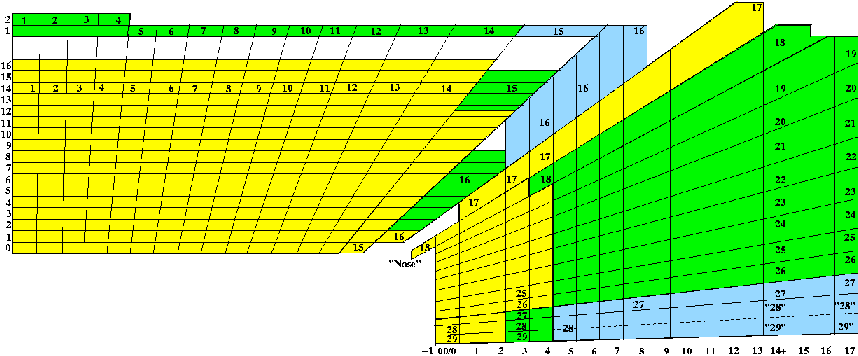
\includegraphics[width=1\textwidth]{pictures/HCAL.pdf}

	\caption[Hadronic calorimeter of CMS]{Schematic view of the towers assembly in barrel and endcap in the r-z plane of the \gls{HCAL}, taken from \cite{CMS2}}
	\label{fig:fig_2_9}
\end{figure}

\subsection*{Magnet}

The superconducting coil is made of niobium-titan alloy, which has a inner diameter of 6.22 m and a length of 13.48. The coil is enclosed in an iron yokes, which gives rise to a magnetic field of 4 Tesla. The barrel part of the iron yoke is 11 long and divided into five rings with a distance of 2.5 along the beam axis, and has a material weight of 6000 tonnes. The end cap of the iron jokes is made of three disk at each side of the detector with a weight of 4600 tonnes.

\subsection*{Muon chambers}

The most outer detector component is the muon detector, which is embedded in the iron yoke. The muon system itself relies for the muon detection on three types of gaseous detectors, the drift tubes, the cathode strip chambers and the resistive plate chambers. In the barrel region, covering the region $|$\gls{eta}$|$ $< 1.2$, 250 drift tube chambers organized in four layers with a distance to the beam pipe of 4-7 meters are installed. To the drift tubes 1 or 2 resistive plates chamber are coupled depending on the layer. The endcap region of the system, covering the region of $|$\gls{eta}$|$ $< 2.4$, 468 cathode strip chambers are installed in both sides of the detector, which are assembled in 4 rings. In the region of $|$\gls{eta}$|$ $< 1.6$  resistive plates chamber are coupled to the cathode strip chambers. Figure \ref{fig:fig_2_10} shows a overview of the muon system.

\begin{figure}[ht]
	\centering
	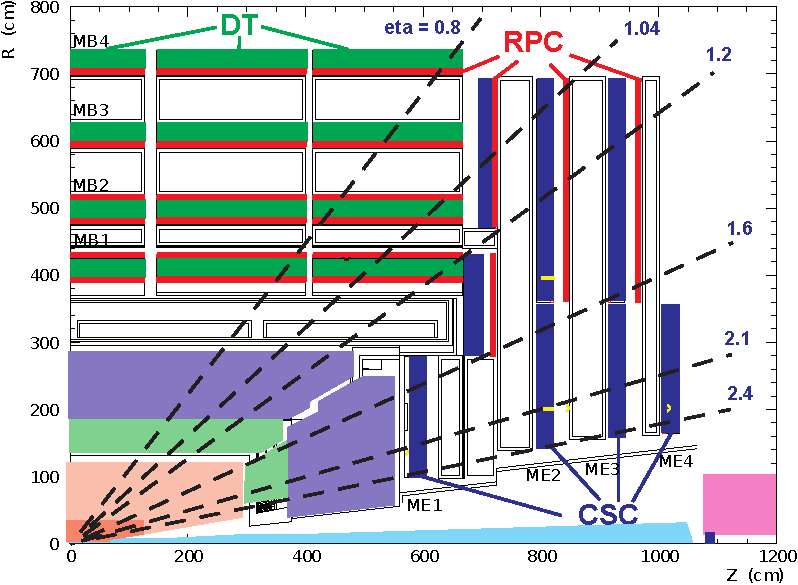
\includegraphics[width=1\textwidth]{pictures/MUON_SYSTEM.pdf}

	\caption[Muon detector system of CMS]{Schematic view of the muon detector system of the r-z plane, where the drift tubes are drawn in green, the resistive plates chamber are drawn in red and the cathode strip chambers are drawn in blue. Taken from \cite{CMS2}}
	\label{fig:fig_2_10}
\end{figure}


\subsection{Trigger system of \gls{CMS}}
\label{sec:section_2_2_3}

The collision rate at the collision point of \gls{CMS} is about 40 Gigahertz, coming from the 25 ns time between the beam bunches, see section \ref{sec:section_2_1_1}. This collision rate at the luminosity of $\mathcal{L} = 10^{34}$ cm$^{-2}$s$^{-1}$  leads to interactions $10^9$ per second. Because the bare amount of data originating from this collisions can neither processed nor saved. Therefore an online selection is done by the \gls{CMS} trigger system \cite{CMS2, TRIGGER}. \\

The first trigger stage is the L1 trigger. This decision of this trigger is taken from the information various local trigger from the detector subsystem, which uses all information recorded of by the calorimeters and the muon system in an event. The second stage is the High Level Trigger \gls{HLT}. Based on the events passing the L1 trigger, the \gls{HLT} decide to keep events on behalf of kinematic variables, which are reconstructed online before the trigger decision. 

\subsection{Particle identification}
\label{sec:section_2_2_4}

The detector components described in the previous section are designed to detect and measure different properties of the particles. Charged particles, like leptons and charged hadrons, have bended trajectories in the magnetic field of \gls{CMS} and leaving hits in the pixel and strip detectors of the tracker system. Neutral particles like photons and neutral hadrons don't leave any track in the tracker system and have a straight trajectory. In the \gls{ECAL} electrons and photons interact with the \gls{PbWO4} and trigger an electromagnetic shower, until the complete energy is deposited. In the \gls{HCAL} all kind of hadrons interact with the brass plates, leading to a cascade of hadron production, until the complete energy is deposited. The muons, which penetrate these sub-detectors losing energy usually only by ionization and leave hits in the muon detector system. Neutrinos can not be measured at all and escape the detector undetected. \\

The bundle of particles, which originating from one object, like a quark or gluon, are jets. There are different algorithms to define and reconstruct jets in \gls{CMS}. Mostly, the anti-kt algorithm is used, counting all particles in a cone with \gls{dR} $= \sqrt{(\Delta \phi)^{2} + (\Delta \eta)^{2}}$.\\ 

From the bending radius of the particles tracks measured in the tracker and for the muons in the muon detector, the transverse momentum \gls{pT} $= \sqrt{p_{x}^{2} + p_{y}^{2}}$ can be measured using 

\begin{equation}
	\label{eq:eq_2_5}
	p_{T} = q\cdot B \cdot R
\end{equation} 

with $q$ as the electric charge of the particle, $B$ the magnetic field flux and R the bending radius of the trajectory. The energy of electrons, photons and hadrons is measured using the energy deposition in the calorimeters. Due to neutrinos and possible \gls{BSM} weakly interacting particles, some energy is not detected. This missing energy measured in the transverse plane (\gls{MET}) is calculated using the fact that in the transverse plane the sum of the momenta of all particles should be zero, due to the protons only having momenta in z-direction. This leads to the formula for \gls{MET}

\begin{equation}
	\label{eq:eq_2_6}
	\vec{E}_{T}^{\text{miss}} = - \sum_{i \in (1, .., n_{\text{meas.}})} \vec{p}_{T}^{i}.
\end{equation}

From the energy and momentum of the visible measured particles, the invariant visible mass distribution \gls{m_vis} of the mother particles can be reconstructed with 

\begin{equation}
	\label{eq:eq_2_6}
	m_{vis} = \sqrt{(E_{1} + E_{2})^2 - (\vec{p}_{1} + \vec{p}_{2})^2}.
\end{equation}


Particles with a short life time, as the $\tau$ lepton, decay into stable particles, which origin from a secondary vertex. To characterize the properties of the particles coming from secondary vertices, the trajectory is extrapolated beyond the secondary vertex and the point of closest approach $d_{0}$ is measured of this extrapolated trajectory and the collision point, see figure \ref{fig:fig_2_11}.

\begin{figure}[ht]
	\centering
	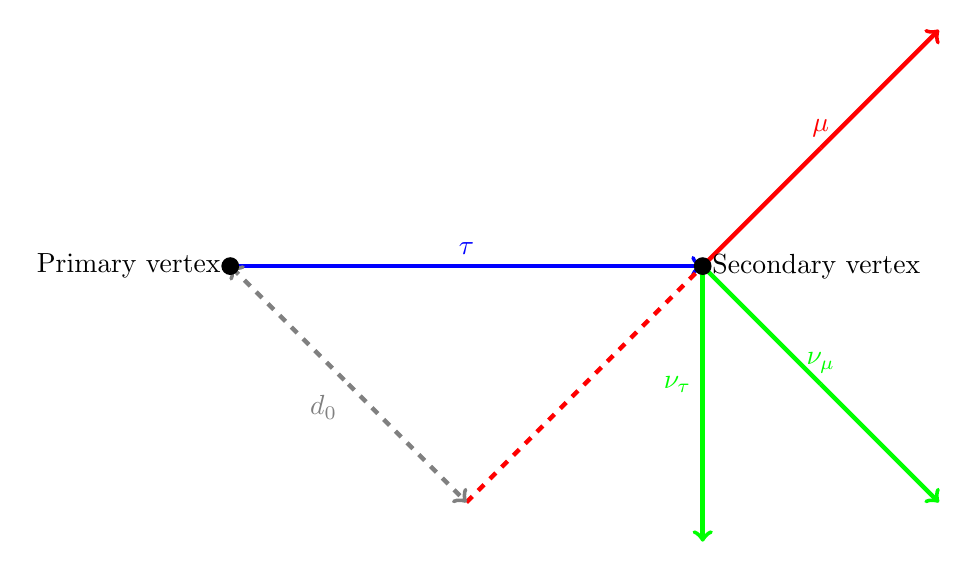
\begin{tikzpicture}
		\draw[blue, ultra thick] (-6,0) -- (-3,0) node[anchor=south] {$\tau$};
		\draw[->, blue, ultra thick] (-6,0) -- (0,0);
		\draw[red, ultra thick] (0,0) -- (1.5,1.5) node[anchor=south] {$\mu$};
		\draw[->, red, ultra thick] (1.5,1.5) -- (3,3);
		\draw[green, ultra thick] (0,0) -- (1.5,-1.5) node[anchor=south] {$\nu_{\mu}$};
		\draw[->, green, ultra thick] (1.5,-1.5) -- (3,-3);
		\draw[green, ultra thick] (0,0) -- (0,-1.5) node[anchor=east] {$\nu_{\tau}$};
		\draw[->, green, ultra thick] (0,-1.5) -- (0,-3.5);
		\draw[red, ultra thick, dashed] (-3,-3) -- (0,0);
		\draw[<-, gray, ultra thick, dashed] (-6,0) -- (-4.5,-1.5) node[anchor=north east] {$d_0$};
		\draw[->, gray, ultra thick, dashed] (-4.5,-1.5) -- (-3,-3);
		\filldraw[black] (-6,0) circle (3pt) node[anchor=east] {Primary vertex};
		\filldraw[black] (0,0) circle (3pt) node[anchor=west] {Secondary vertex};
	\end{tikzpicture}
	\caption[Construction of point of closest approach]{Construction for measuring the point of closest approach $d_{0}$ of the muon trajectory to the collision point}
	\label{fig:fig_2_11}
\end{figure}



\clearpage{\pagestyle{empty}\cleardoublepage}

\appendix

\chapter*{Acronyms}
\addcontentsline{toc}{chapter}{Acronyms}
\begin{acronym}[Bash]
	\acro{SM}{Standard Model of Particles Physics}
	\acro{QFT}{Quantum field theory}
	\acro{QED}{Quantum electrodynamics}
	\acro{QCD}{Quantum chromodynamics}
	\acro{LFV}{Lepton flavour violation}
	\acro{BSM}{Beyond the Standard Model of Particle Physics}
	\acro{LHC}{Large Hadron Collider}
	\acro{CMS}{Compact Muon Solenoid}
	\acro{TeV}{Tera electron volt, $1 \text{ TeV} = 1.6 \cdot 10^{-7}$ J}
	\acro{CERN}{European Organization for Nuclear Research, abbreviation from Conseil européen pour la recherche nucléaire}
	\acro{ATLAS}{A Toroidal LHC Apparatus}
	\acro{LHCb}{Large Hadron Collider beauty}
	\acro{ALICE}{A Large Ion Collider Experiment}
	\acro{PDF}{Parton density function}
\end{acronym}

\clearpage{\pagestyle{empty}\cleardoublepage}

\bibliographystyle{packages/bibstyle.bst}
\bibliography{bibliography.bib}
\addcontentsline{toc}{chapter}{Bibliography}

\end{document}
